% !TEX ROOT = ../ersti.tex
\section{Rahmenprogramm}
\subsection{Wanderungen}
An den Wochenenden (Samstag 03.10. und Sonntag 11.10.) werden wir jeweils eine
kleine Wanderung unternehmen und im Anschluss gemütlich grillen oder
picknicken. Die erste Tour führt voraussichtlich auf den Heiligenberg, die
zweite auf den Königstuhl -- die beiden Hausberge (Hügel) Heidelbergs. Am
Anschluss an die erste Tour werden wir an der Thing-Stätte\footnote{alle Infos
hierzu während der Wanderung erfragen} grillen, im Anschluss an die zweite Tour
im Schlossgarten Picknicken.  Bringt euch für das Picknick alles wichtige
selber mit.

\noindent\emph{Wir treffen uns jeweils um 11 Uhr am Bismarckplatz.}

\subsection{Spieleabende}
Das Abendprogramm wird spontan entschieden, meist handelt es sich um Gesellschaftsspiele -- bringt auf jeden Fall eigene Spiele mit, was auch immer ihr unter Spielen versteht. Manchmal wird auch zusätzlich gegrillt, wenn von der Wanderung noch Reste übrig geblieben sind.

Bisher sind Gesellschaftsspiele super angekommen (da lernt man sich kennen), Alternativvorschläge sind natürlich trotzdem immer gern gesehen, falls euch etwas einfällt meldet euch doch einfach, schließlich wird das Ganze ja für euch veranstaltet.

\subsection{Brunch}
Am ersten Sonntag des Vorkurses (4. Oktober) bereiten wir euch einen
wunderschönen, leckeren Brunch in der Reinen Mathe (\gls{INF} 288), der das
beste Frühstück wird, das ihr in euren ersten zwei Wochen bekommen werdet.
Bringt bitte euer eigenes Geschirr/Besteck mit, damit wir Plastikquatsch
sparen.

\iffalse
\subsection{Nicht nur die Fachschaft macht interessantes Programm...}
In den ersten Semesterwochen gibt es eine Vielzahl von Angeboten (auch) für Erstsemester. Hier eine Auswahl:
\begin{itemize}
\item Montag 13.10.2014, 9:00–12:00 Uhr, \gls{INF} 252, offizielle Erstsemesterbegrüßung des Rektors mit „Studienauftaktmesse“ in der Mensa (\gls{INF} 304), bei der sich viele studentische Gruppierungen vorstellen
\item Freitags, 19:00, ZEP, Zeppelinstraße 1: Vokü
\item Sonntags, im Sep. 20:00 / ab Okt. 19:00, Cafe Gegendruck, Fischergasse 2: Vokü
%\item Di, 04.10.2011, 18:00, Universitätsplatz: Antifaschistischer Stadt\-rund\-gang \\ Die Antifaschistische Initiative nimmt euch mit in die dunkelbraune Vergangenheit und Gegenwart Heidelbergs. Zwar wird an der Uni nicht mehr "Deutsche Physik" gegen "jüdische Umtriebe" wie die Allgemeine Relativitätstheorie betrieben, aber immer noch wettert die Deutsche Bur\-schen\-schaft, der auch zwei Heidelberger Bur\-schen\-schaf\-ten angehören, gegen "außereuropäische Gesichtsmorphologie" in ihren Reihen. Der Rundgang führt euch zu verschiedenen Schauplätzen faschistischer und antifaschistischer Stadtgeschichte.
% zu früh.. \item \textbf{Mi, 05.10.2011, 20:00, Heinrich-Fuchs-Str. 85: Vernetzungstreffen zur Nutzung der US-Flächen ab 2015} \\ Nach dem Abzug der US-Truppen 2015 wird ein gigantisches Areal in Heidelberg frei. Wofür soll es genutzt werden? Alle Menschen mit Ideen für alternative Wohnprojekte, Kulturprojekte, Soziale Zentren u.v.m. sind hier willkommen.
%\item Do, 06.10.2011, 16:00, Mensavorplatz: Kakipflaumen und Minikiwis - Obstbäume im Neuenheimer Feld \\ Was tun, wenn im Geldbeutel wieder Flaute ist, oder man einfach scharf auf ein paar neue Geschmackserlebnisse ist? Das Neuenheimer Feld kann seine Vergangenheit als Obstanbaugebiet nicht verleugnen und auch die Uni hat das reichhaltige Angebot um ein paar ganz besondere Leckerbissen erweitert. Alle klassischen Obstarten sind vertreten, daneben aber auch Exoten wie mehrere Kiwiarten, Lotuspflaumen, Weissdornfrüchte, Baumgurken, Feigen, u.v.m. Der Herbst ist die beste Zeit, diese Vielfalt zu erleben, was wir auf einem ca. 2-stündigen Spaziergang über den Campus versuchen wollen.\\ Aber Vorsicht: Obwohl einem das Obst im Feld uneingezäunt und verlockend quasi in den Mund wächst, sind die Bäume allesamt Eigentum des Landes Baden-Württemberg. Auf dem Campus wachsen zudem auch zahlreiche giftige Früchte. Für Vergiftungen bei Selbstversuchen wird keine Haftung übernommen.
\item Donnerstags im Semester, 18:00, Cafe da lang, IBW, Akademiestr. 3: Lehramts-Cafe. Infos zum äußerst empfehlenswerten Programm des Lehramts-Cafes bekommt ihr auf der Mailingliste \footnote{\url{https://fsk.uni-heidelberg.de/mailman/listinfo/lehramtscafe}} oder über Aushänge am Fachschafts-Brett.
\end{itemize}
\fi

\marginpar{
    \centering{
        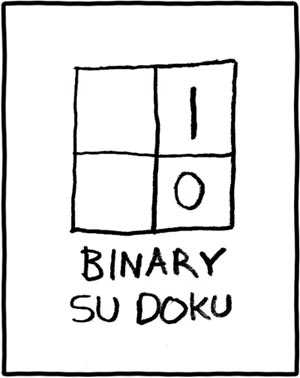
\includegraphics[width=3cm]{bilder/su_doku.png}\\
    }
}
